%
% $RCSfile: application_and_domain.tex,v $
%
% Copyright (C) 2002-2008. Christian Heller.
%
% Permission is granted to copy, distribute and/or modify this document
% under the terms of the GNU Free Documentation License, Version 1.1 or
% any later version published by the Free Software Foundation; with no
% Invariant Sections, with no Front-Cover Texts and with no Back-Cover
% Texts. A copy of the license is included in the section entitled
% "GNU Free Documentation License".
%
% http://www.cybop.net
% - Cybernetics Oriented Programming -
%
% http://www.resmedicinae.org
% - Information in Medicine -
%
% Version: $Revision: 1.1 $ $Date: 2008-08-19 20:41:05 $ $Author: christian $
% Authors: Christian Heller <christian.heller@tuxtax.de>
%

\subsection{Application and Domain}
\label{application_and_domain_heading}
\index{Application and Domain}
\index{Domain Knowledge}
\index{Application Functionality}
\index{Tools \& Materials Approach}
\index{Active Application (Tool)}
\index{Passive Domain Data (Material)}
\index{System Family Engineering}
\index{Domain Engineering}
\index{DE}
\index{Application Engineering}
\index{AE}
\index{Domain-Application- versus System-Knowledge Separation}
\index{User Interface}
\index{UI}
\index{Database}
\index{DB}
\index{Model View Controller Pattern}
\index{MVC}
\index{Data Mapper Pattern}
\index{Structured Query Language}
\index{SQL}
\index{Database Management System}
\index{DBMS}
\index{Enterprise Java Bean}
\index{EJB}
\index{Middleware}
\index{Translator Pattern}
\index{Data Transfer Object Pattern}
\index{DTO}

Over the years, it has turned out to be helpful in software design, to separate
\emph{Domain Knowledge} from \emph{Application Functionality}. In one-or-another
form, the architectural patterns (section \ref{architectural_heading})
\emph{Layers}, \emph{Domain Model} and \emph{Model View Controller} (MVC) all
suggest to apply this principle. Figure \ref{logical_figure} showed a typical
example of a system with logical layers, among them a domain layer containing
business logic.

The \emph{Tools \& Materials} approach of section \ref{tool_and_material_heading}
talks of \emph{active} applications (tools) working on \emph{passive} domain
data (material). And also \emph{System Family Engineering}, as mentioned at the
beginning of section \ref{domain_engineering_heading}, is based on a separate
treatment of domain and application, in form of \emph{Domain Engineering} (DE)
and \emph{Application Engineering} (AE).

An often neglected fact of these approaches is that not only the domain, but
also the application contains important business knowledge. Figure
\ref{separation_figure} tries to demonstrate this by organising typical
software patterns (section \ref{pattern_heading}) and system functionality into
two orthogonal pairs of layers. The \emph{User Interface} (UI), for example, is
mostly assigned to the application layer, yet since it is clearly tailored for
a specific business domain, it be better assigned to a knowledge layer,
together with the corresponding domain models. And the logic behind a UI, if
not contained in the UI itself, is often put in a \emph{Controller} which
belongs to the application-, not the domain layer. But because a controller's
task is the management of general functionality like the processing of signals
(events) and communication, which are not application-specific, it be better
sorted into a low-level system layer. It is true that controllers often contain
some application logic; but that in turn belongs to the high-level knowledge
layer above it.

\begin{figure}[ht]
    \begin{center}
        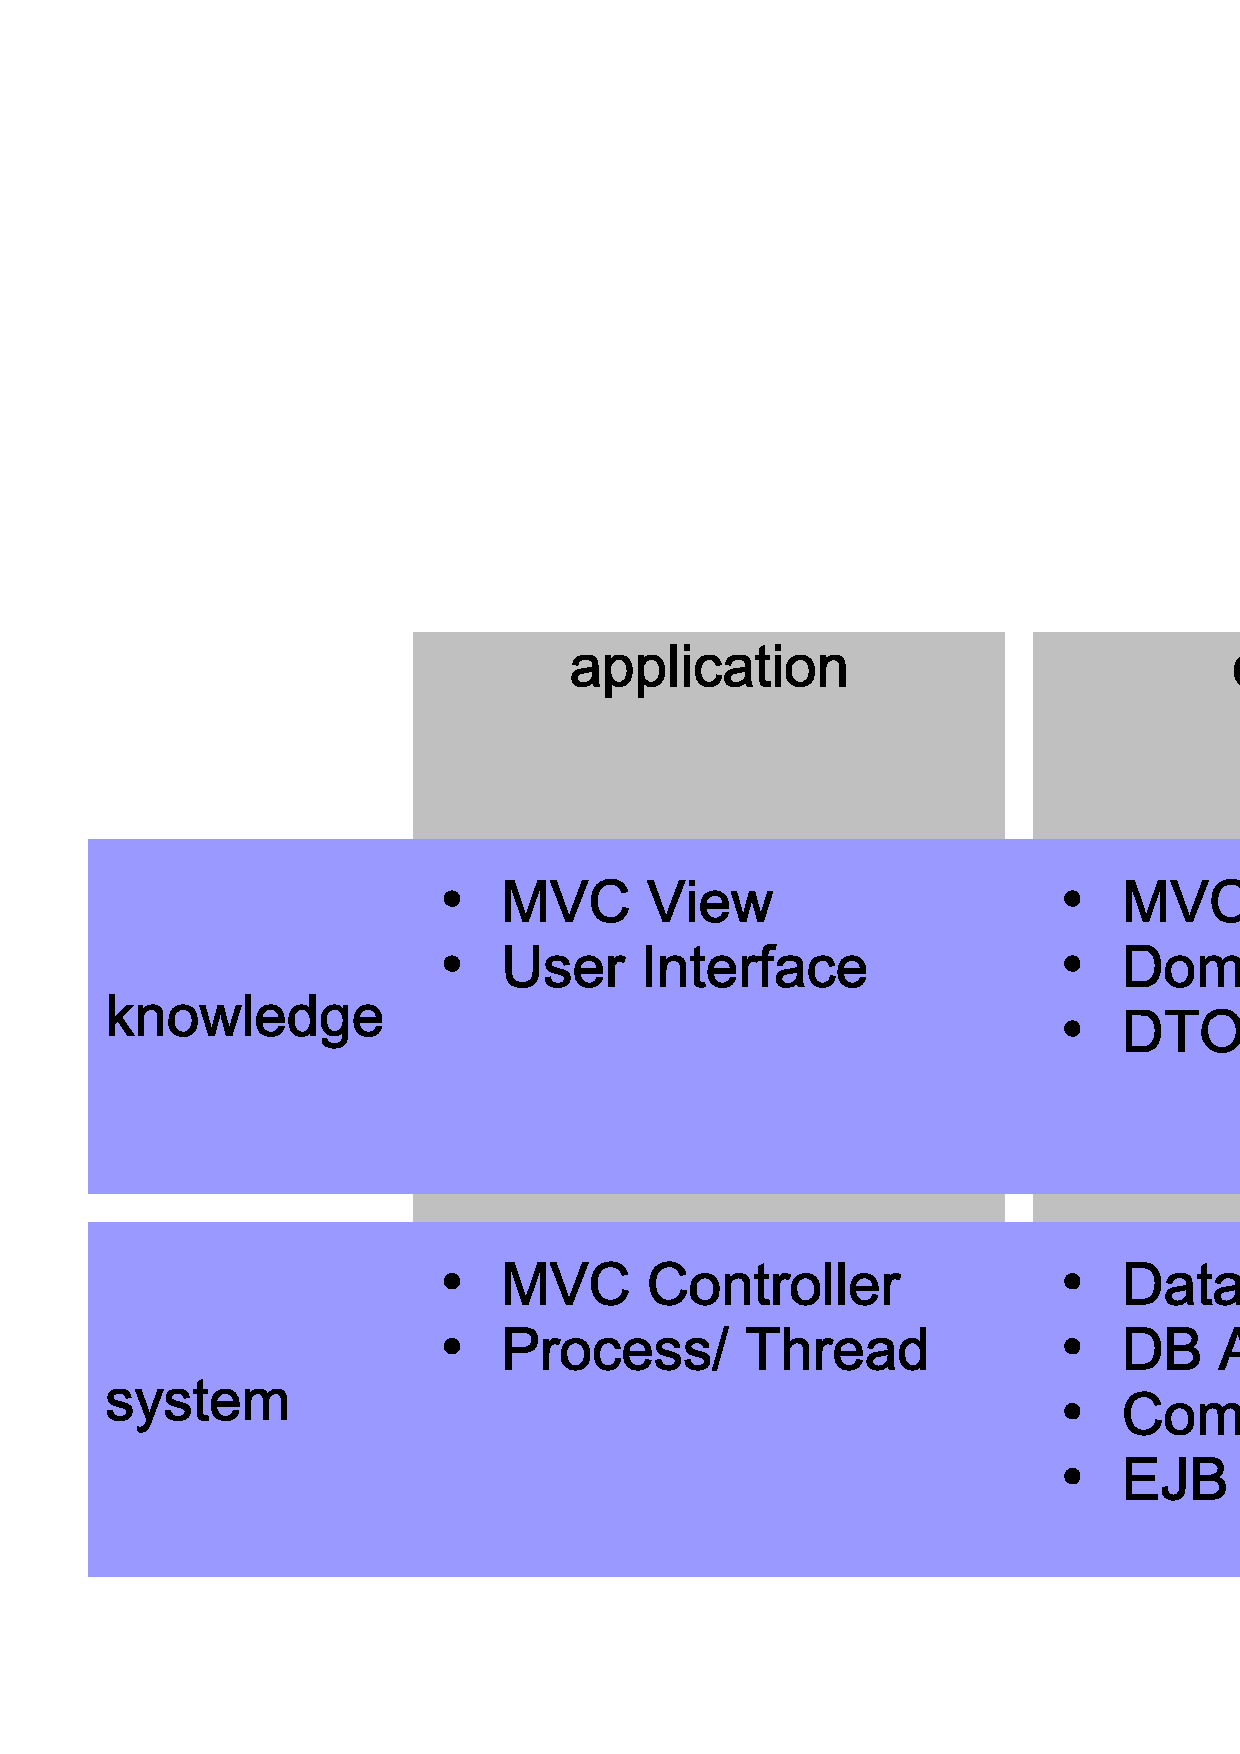
\includegraphics[scale=0.3,angle=-90]{graphic/separation.pdf}
        \caption{Domain-Application- versus System-Knowledge Separation}
        \label{separation_figure}
    \end{center}
\end{figure}

Similarly, the domain often contains functionality which actually does belong
into the application process: \emph{Database} (DB) access is handled by help of
patterns like the \emph{Data Mapper} (section \ref{data_mapper_heading}), in
which the mapper objects contain \emph{Structured Query Language} (SQL) code to
connect to a \emph{Database Management System} (DBMS);
\emph{Enterprise Java Beans} (EJB), which should better be pure domain objects,
imitate a \emph{Middleware} providing persistence- or other communication
mechanisms, which originally have nothing to do with the business knowledge
they contain.

It is precisely this \emph{Mixup} of responsibilities between an application
system and its domain knowledge, that leads to multiple inter-dependencies and
hence unflexibility within a system. Instead, a separation should be made
between active \emph{System Control} and passive \emph{Knowledge}. A UI's
appearance would then be treated as domain knowledge, just as the logic of the
functions called through it. A data mapper would be transformed into a simple
\emph{Translator} -- similar to a \emph{Data Transfer Object} (DTO) (section
\ref{data_transfer_object_heading}) -- that knows how to convert data from one
domain model into another; its DBMS access functionality, however, would be
extracted and put into the system layer. More on that in chapter
\ref{state_and_logic_heading}. Monstrosities like EJBs would likewise be opened
up and parted into their actual domain knowledge, and all the other mechanisms
around -- the latter being moved into the low-level system layer.

To sum up this thought: The essential realisation here is that hardware-close
mechanisms like the ones necessary for data input/ output (i/o), enabling
inter-system communication, should be handled in an active system layer which
was started as process on a computer, and \emph{not} be merged with pure,
passive domain knowledge. Application logic which is traditionally held in
controller objects of the application layer, and other business data models
should rather belong to a high-level knowledge layer.

In chapter \ref{cybernetics_oriented_interpreter_heading}, this work introduces
an interpreter providing low-level functionality. High-level knowledge, on the
other hand, may be modelled in the language defined in chapter
\ref{cybernetics_oriented_language_heading}.
